% %\documentclass[oneside,final,14pt]{article}
\documentclass[14pt,oneside,final]{extreport}
\usepackage[utf8]{inputenc} 
\usepackage[english,russian]{babel}
\usepackage{vmargin}
\setpapersize{A4}
\setmarginsrb{20mm}{20mm}{20mm}{20mm}{0pt}{0mm}{0pt}{13mm}
\usepackage{indentfirst}
\usepackage{pscyr} % Нормальные шрифты
\DeclareUnicodeCharacter{00A0}{~}
\usepackage[T2A]{fontenc} % Поддержка русских букв
\usepackage{url}
\usepackage{tabularx}
\newcolumntype{Z}{>{\centering\let\newline\\\arraybackslash\hspace{0pt}}X} %новый тип столбца для таблицы

\usepackage[nooneline]{caption} 
\captionsetup[table]{justification=raggedleft} 
\captionsetup[figure]{justification=centering,labelsep=endash} 

\usepackage{titlesec}

\usepackage{subcaption}
   
\titleformat{\chapter}[display]
{\filright\large}
{} % %{\MakeUppercase{\chaptertitlename} \thechapter}
{8pt}
{\bfseries}{}
     
\titleformat{\section}
{\normalsize\bfseries}
{\thesection}
{1em}{}
     
\titleformat{\subsection}
{\normalsize\bfseries}
{\thesubsection}
{1em}{}
     
% Настройка вертикальных и горизонтальных отступов
\titlespacing*{\chapter}{0pt}{-30pt}{8pt}
\titlespacing*{\section}{\parindent}{*4}{*4}
\titlespacing*{\subsection}{\parindent}{*4}{*4}
    
% всавка изображений
\ifx\pdfoutput\undefined
\usepackage{graphicx}
\else
\usepackage[pdftex]{graphicx}
\fi
% сквозная нумерация
\usepackage{chngcntr}
\counterwithout{figure}{chapter}

\renewcommand{\thefigure}{\arabic{figure}}
\usepackage[tableposition=top]{caption}
\usepackage{subcaption}
\DeclareCaptionLabelFormat{gostfigure}{Рисунок #2}
\DeclareCaptionLabelFormat{gosttable}{Таблица #2}
\DeclareCaptionLabelSeparator{gost}{~---~}
\captionsetup{labelsep=gost}
\captionsetup[figure]{labelformat=gostfigure}
\captionsetup[table]{labelformat=gosttable}
\captionsetup{figurewithin=none, tablewithin=none} %сквозная нумерация таблиц
\renewcommand{\thesubfigure}{\asbuk{subfigure}}

\linespread{1.3}
\usepackage[toc,page]{appendix}
    \renewcommand\appendixname{Приложение}
    \makeatletter
    \def\redeflsection{\def\l@section{\@dottedtocline{1}{1.5em}{7.8em}}}
    \renewcommand\appendix{\par
    \setcounter{section}{0}%
    \setcounter{subsection}{0}%
    \def\@chapapp{\appendixname}%
    \addtocontents{toc}{\protect\redeflsection}
    \def\thesection{\appendixname\hspace{0.2cm}\@arabic\c@section}}
    \makeatother


\sloppy


\begin{document}
	\renewcommand*\contentsname{\hfill Содержание \hfill}
	\tableofcontents
	
	\chapter{Введение}
	Эксплуатационные характеристики изделий машиностроения в большой мере зависят от качества изготовления деталей, составляющих изделие. Качество изготовления определяется степенью соответствия параметров готовой детали и параметров, достижение которых требуется документацией. В роли такого параметра может выступать точность изготовления геометрических размеров, определяемая допуском. 
	
	Погрешности различных видов препятствуют абсолютно точному воспроизведению заданных параметров. Например, на точность изготовления деталей влияют погрешности базирования, измерения, настройки инструмента и т.д. При обработке нежестких деталей на первый план выходят погрешности, связанные с деформацией самой детали.
	
	Рассмотрим пример обработки тонкостенной детали в трехкулачковом патроне токарного станка. Схема обработки изображена на рисунке~\ref{fig:1}. Цифровыми сносками обозначены: 1~-~кулачок патрона, 2~-~цилиндрическая заготовка, 3~-~токарный резец. До начала обработки деталь находится в недеформированном состоянии (рисунок~\ref{fig:1a}). После закрепления детали силы, действующие со стороны кулачков, деформируют заготовку таким образом, что профиль заготовки отличается от идеально цилиндрического (рисунок~\ref{fig:1b}). Дополнительно заготовка деформируется под действием силы резания, а также в связи с нагревом. В процессе резания инструмент неравномерно снимает припуск по окружности заготовки (рисунок~\ref{fig:1c}). После окончания обработки и снятия усилий закрепления отклонение от круглости заготовки достигает величин, сравнимых с величиной допуска и в зависимости от конкретных условий может превышать его (рисунок~\ref{fig:1d}).
	
	\begin{figure*}[t!]
	    \centering
	    \begin{subfigure}[t]{0.5\textwidth}
	        \centering
        	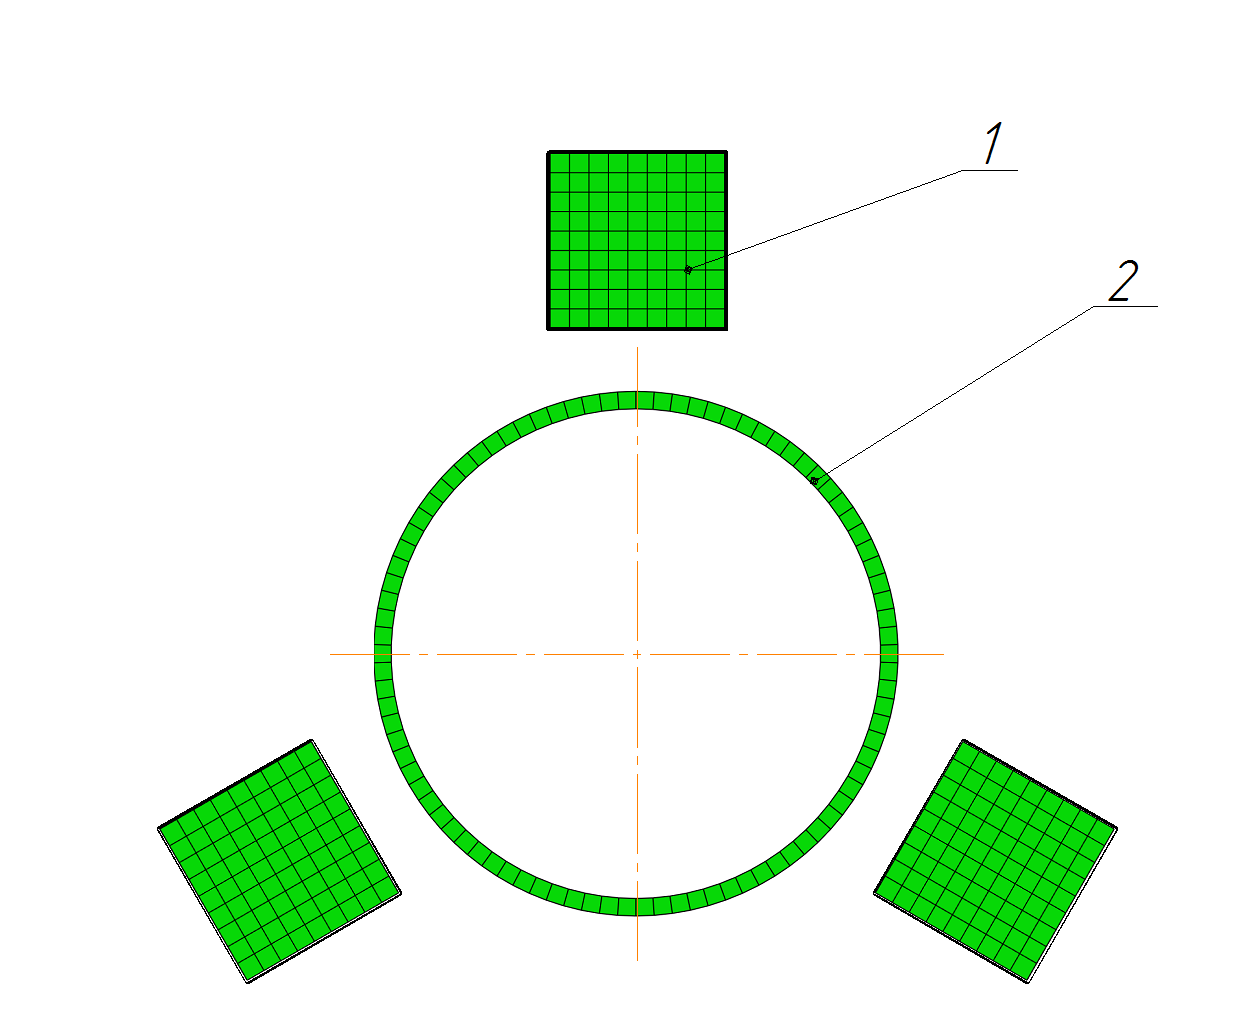
\includegraphics[scale=0.25]{img/fig1a}
	        \caption{До закрепления} \label{fig:1a}
	    \end{subfigure}%
	    ~ 
	    \begin{subfigure}[t]{0.5\textwidth}
	        \centering
        	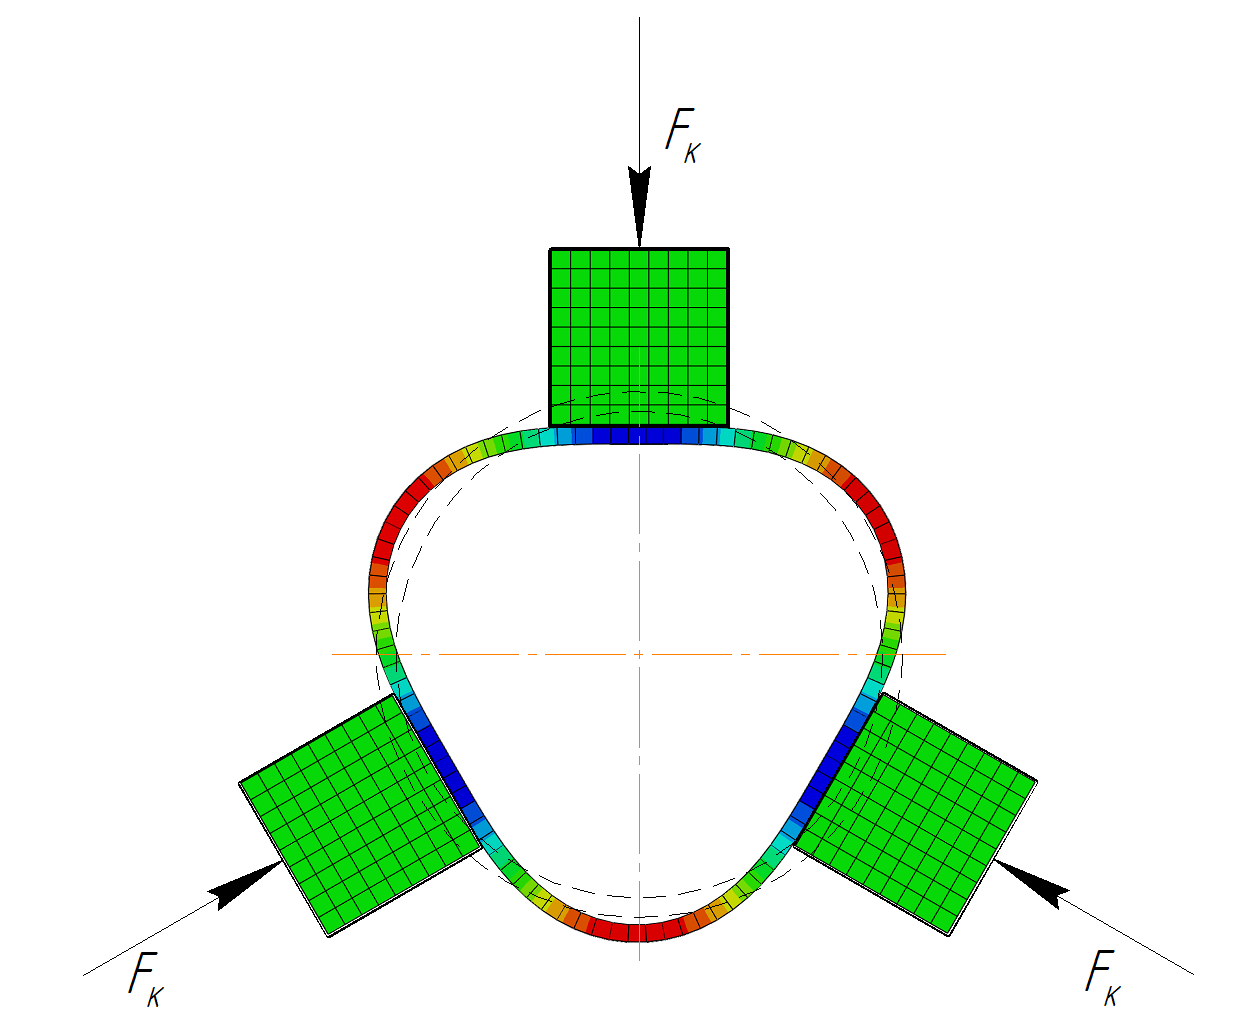
\includegraphics[scale=0.25]{img/fig1b}
        	\caption{Закрепленная заготовка} \label{fig:1b}
	    \end{subfigure}
	    
   	    \begin{subfigure}[t]{0.5\textwidth}
   	        \centering
           	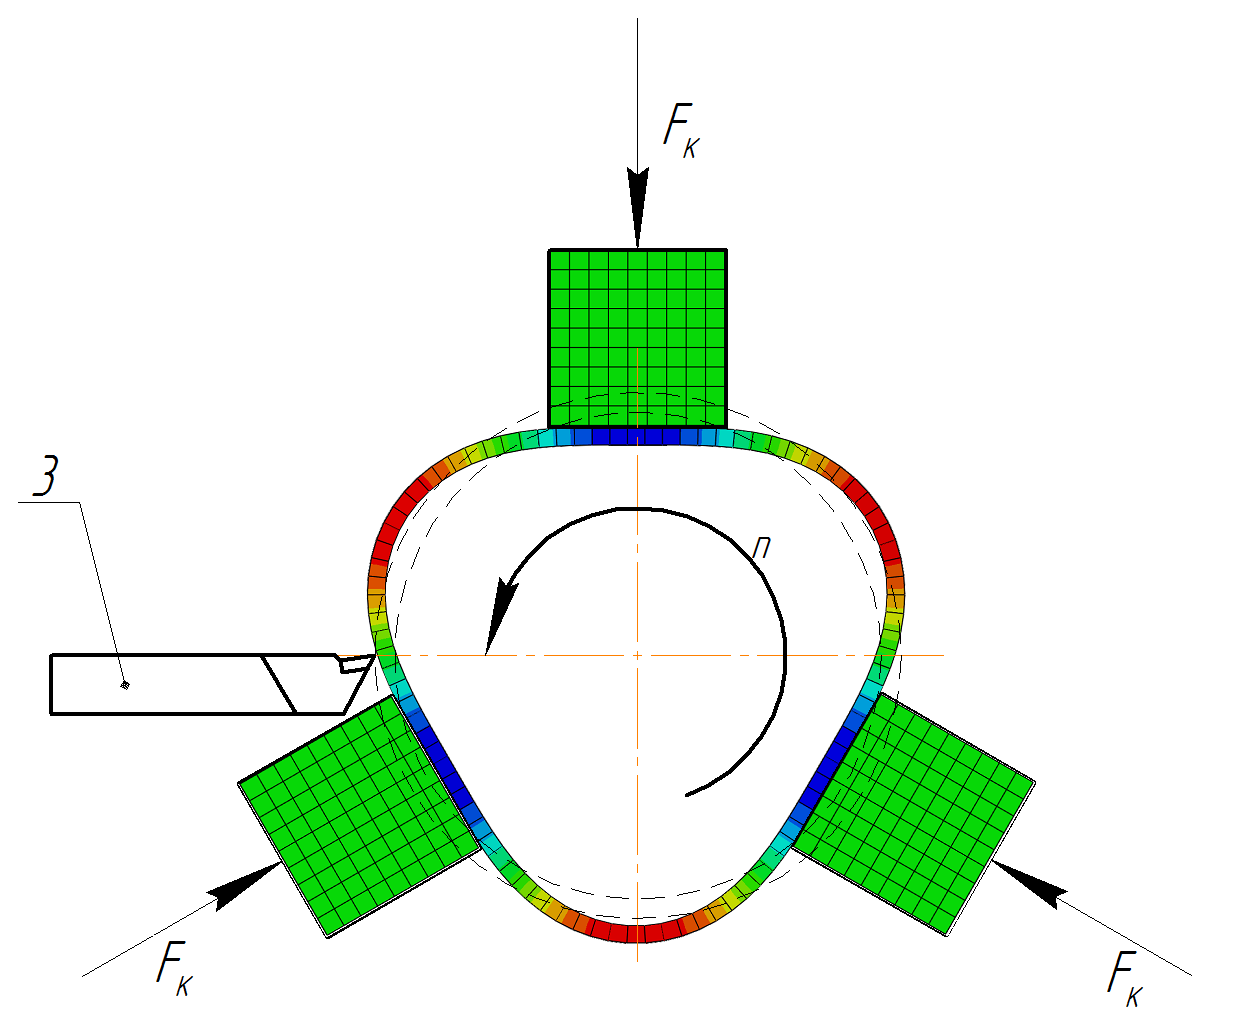
\includegraphics[scale=0.25]{img/fig1c}
           	\caption{Обработка} \label{fig:1c}
   	    \end{subfigure}%
   	    ~
   	    \begin{subfigure}[t]{0.5\textwidth}
   	       	\centering
   	        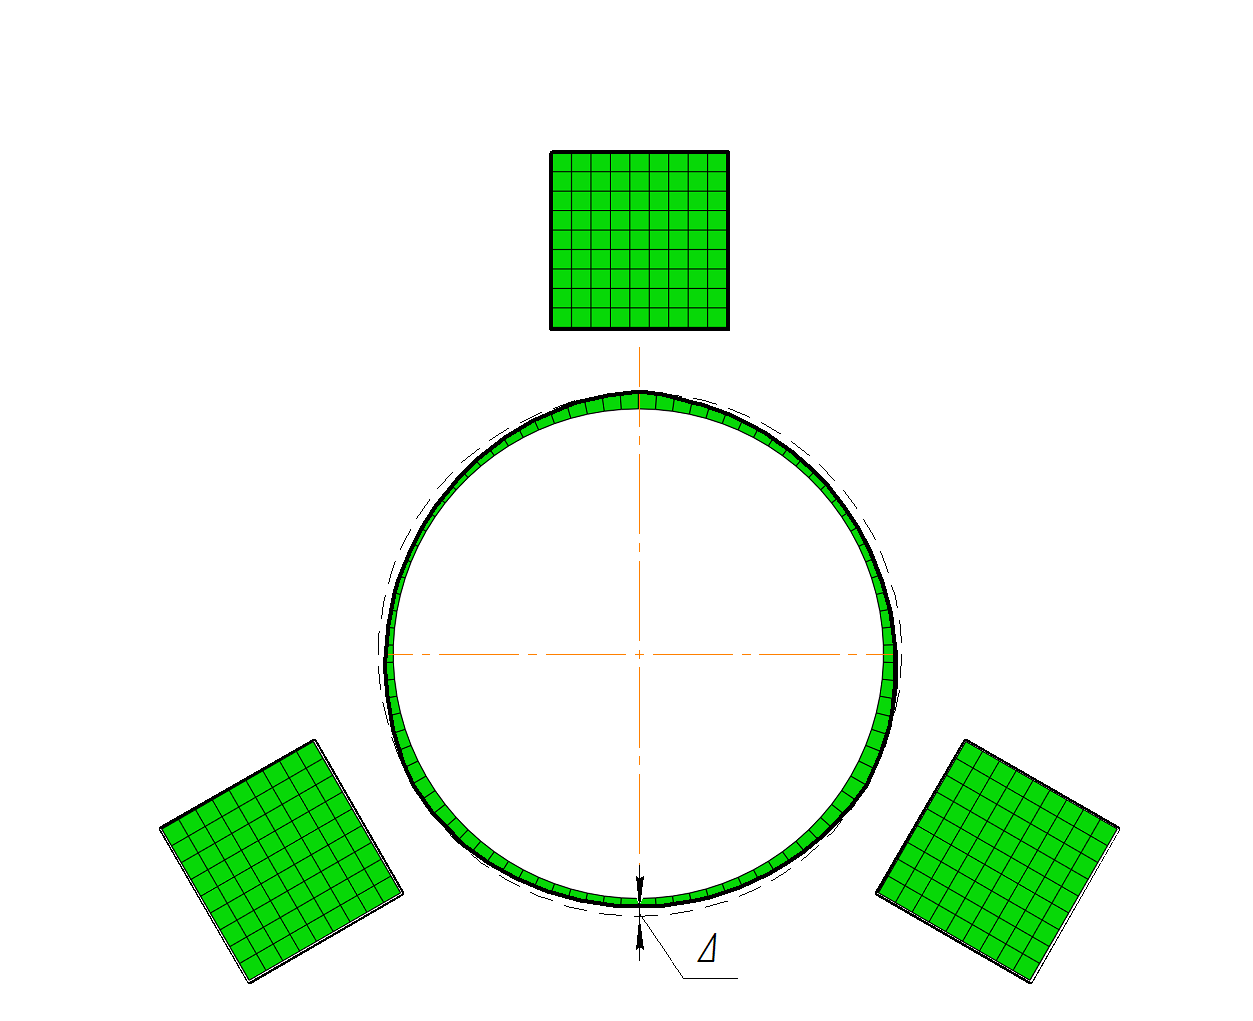
\includegraphics[scale=0.25]{img/fig1d}
   	    	\caption{Результат} \label{fig:1d}
	   	\end{subfigure}
	    \caption{Обработка тонкостенной заготовки} \label{fig:1}
	\end{figure*}


	На практике в случае обработки нежестких деталей применяется специальное технологическое оборудование, позволяющее уменьшить возникающие деформации. Использование сырых кулачков, растрачиваемых под диаметр заготовки - один из способов уменьшения деформаций закрепления. После растачивания кулачок охватывает деталь по большей площади. Также используется обработка с технологическим заполнителем (например, легкоплавким материалом), который увеличивает жесткость детали на время обработки и выплавляется после окончания обработки. Вариант обработки на нормативных режимах резания в специальных приспособлениях привлекателен тем, что он позволяет применять апробированные технологические процессы. Однако, необходимость создания при этом специальных приспособлений требует значительных материальных, производственных и временных затрат. Это удорожает технологическую подготовку производства и увеличивает её сроки. 

	Ввиду указанных ограничений на существующие способы обработки, предлагается рассмотреть еще один метод - подбор режимов обработки и условий закрепления таким образом, чтобы обеспечить изготовление размеров в рамках допуска. Предполагается, что такой метод может найти применение прежде всего в единичном и мелкосерийном производстве, располагающим, как правило, только универсальным оборудованием. Суть подхода заключается в том, чтобы заранее, на этапе разработки технологической документации, определить режимы резания, менее эффективные с точки зрения производительности, но оптимальные с точки зрения точности изготовления. С уменьшением сил резания уменьшаются и деформации заготовки, а также требуемые усилия закрепления, но с другой стороны, увеличивается время обработки.  Подобрав баланс между скоростью и точностью обработки, технолог имеет возможность назначить режимы резания, приемлемые для изготовления заданной детали без привлечения дополнительной технологической оснастки.  Достоинством такого подхода является меньшая ресурсоёмкость и продолжительность технологической подготовки производства. Однако, данный подход в настоящее время ещё не получил достаточного научного обоснования и, как следствие, не поддержан методическими рекомендациями, необходимыми для его применения в промышленных масштабах \cite{article:zhargalova}.
	
	Для поддержки решения о назначении режимов резания предлагается разработать информационную систему, позволяющую анализировать деформации заготовки при заданных геометрических параметрах и режимах резания. Такой инструмент можно использовать для последовательной проверки ряда значений параметров процесса и выбора наиболее рациональных. 
	
	Система, спроектированная в соответствии с современными тенденциями в разработке ПО станет эффективным инструментом для назначения режимов обработки. Объектно-ориентированная модульная архитектура такой системы позволит расширять её функционал в случае возникновения новых требований к применению системы, а независимость от конкретной операционной системы позволит легко внедрить такие системы в процесс разработки технологической документации на предприятиях безотносительно конкретной существующей информационной среды.
	
	
	\chapter{Техническое задание}	
	
	\section{Основания для разработки}
	Основанием для разработки системы являются документы:
	\begin{enumerate}
	\item Задание на выполнение дипломного проекта
	\item Календарный план на выполнение дипломного проекта
	\end{enumerate}
	
	\section{Назначение разработки}
	    Функциональным назначением разработки является обеспечение интегрированной рабочей среды для гибкого моделирования процессов деформирования тонкостенных заготовок в процессе их токарной обработки. Под гибкостью понимается возможность изменения параметров процесса в зависимости от расчетного случая и конфигурации заготовки. Эксплуатационным назначением является обеспечение инструментального средства для последовательного определения рациональных режимов резания тонкостенных заготовок и автоматизация сопутствующих расчетов.
	
	\section{Требования к функциональным характеристикам}
	    Система информационной поддержки должна обеспечивать выполнение следующих функций:
	Расчет деформаций тонкостенной заготовки при токарной обработке с закреплением в кулачковом патроне.
	Автоматизация необходимых сопутствующих расчетов (режимов резания)
	Изменение параметров рассматриваемого процесса: геометрии заготовки  и оснастки и значений силовых факторов (силы резания и закрепления)
	Представление результатов расчета в виде графиков или таблиц деформаций
	Генерация отчета по результатам расчета
	Вывод дополнительных информационных отладочных сообщений 
	\section{Требования к надежности}
	    Разрабатываемая система должна обеспечивать надежную работу в условиях ошибочного пользовательского ввода.
		\section{Условия эксплуатации}
	    Температура окр. среды, влажность, давление и т.д
		\section{Требования к составу и параметрам технических средств}
	    ОЗУ, ПЗУ, монитор и т.д.
		\section{Требования к информационной и программной совместимости}
	Windows, Linux, и т.д.
	\section{Требования к маркировке и упаковке}
	     Не предъявляются
	\section{Требования к транспортированию и хранению}
	    Не предъявляются
	\section{Требования к программной документации}
	    Не предъявляются
		\section{Технико-экономические показатели}
	    ? ? ?
		\section{Стадии и этапы разработки}
	    ? ? ?
	\section{Порядок контроля и приемки}
	    ? ? ?
		\section{Приложения}
	    ? ? ?
		\section{Предпроектное исследование}
	    ? ? ?
	\chapter{Разработка концепции автоматизированной системы}
	\section{Принцип моделирования}
	Согласно техническому заданию система должна обеспечить расчет деформаций тонкостенной заготовки в процессе токарной обработки. Токарная обработка характеризуется большим разнообразием возможных вариантов осуществления в зависимости от обрабатываемой поверхности и способа закрепления. Разработать и запрограммировать адекватную модель, основанную исключительно на математическом представлении известных теоретических закономерностях сопротивления материалов для каждого из возможных вариантов - чрезвычайно сложная задача с технической точки зрения. 
	
	Известно, что современные CAE системы позволяют успешно решать задачи определения деформаций и напряжений для объектов практически неограниченной сложности благодаря использованию метода конечных элементов. После разбиения рассматриваемых объектов на конечные элементы определенного типа и наложении ограничений на эти элементы согласно закономерностям предметной области задача сводится к решению системы из большого количества уравнений. Успех решения полученной системы уравнений как правило определяется только отведенным на решение временем работы ЭВМ. 
	
	Тем не менее, сама по себе реализация метода конечных элементов в разрабатываемом продукте не возможна из-за большой трудоемкости и требует огромной исследовательской и проектной работы целого коллектива профессионалов. Таким образом, наилучшим выходом из сложившейся ситуации представляется использование готовой CAE системы. Применение системы МКЭ расчета возможно, если она отвечает следующим трем основным требованиям:
	\begin{enumerate}
	\item Предоставляет возможность расчета заранее составленной модели под управлением внешнего процесса операционной системы (в роли которого будет выступать разрабатываемая система анализа деформаций)
	\item Имеет механизмы параметризации модели. В наилучшем случае параметризация должна достигаться благодаря выполнению пользовательских сценариев.
	\item Позволяет получить результат расчета в виде графиков, диаграмм напряжений и деформаций а также в числовом виде для каждого элемента модели.
	\end{enumerate}
		


	В рамках перечисленных соображений можно сформулировать концепцию системы следующим образом. На первом этапе система собирает информацию о значениях параметров модели через графический пользовательский интерфейс. По завершению ввода функция системы состоит в формировании задания для используемой готовой CAE системы. На этапе подготовки задания производится дополнительный расчет необходимых величин, если они не были непосредственно указаны на первом этапе и могут быть получены расчетным путем. Третий этап состоит в вызове расчетного ядра CAE системы по сформированному заданию. По завершению обработки модели разрабатываемая система агрегирует результаты и отображает их пользователю, при необходимости генерируя отчет.

	Таким образом, основная идея состоит в расчете модели обработки с использованием сторонней CAE системы. Предполагается, что роль разработчика моделей будет выполнять эксперт, как правило не являющийся пользователем системы. В задачи эксперта входит описание нового расчетного случая при помощи инструментов, предоставляемых конкретной выбранной системой МКЭ расчета и другие необходимые работы по подготовке системы. Готовая модель предоставляется в распоряжению пользователю, в задачи которого входит выбор наиболее подходящей модели из множества имеющихся и её загрузка в разрабатываемую систему поддержки.

	\section{Принцип модульности}
	Уже на этапе формулирования концепции системы становиться видна её большая сложность. Для того чтобы сохранить контроль над расширяющейся по мере разработке системы и не допустить её деградации следует определиться с принимаемыми для этого мерами и также включить их в концепцию системы, т.к. принимаемые меры коренным образом повлияют на процесс проектирования. 
	
	В соответствии с накопленным мировым опытом в разработке программного обеспечения одним из наиболее жизнеспособных способов контроля сложности является разработка приложения в соответствии с принципами  объектно-ориентированного программирования. Во-первых,  ООП методология позволяет добиться большого процента повторного использования кода благодаря принципам наследования и полиморфизма \cite{Shildt}. Во-вторых, принципы абстракции и инкапсуляции облегчают задачу программиста т.к. существенно ограничивают область кода, который влияет на рассматриваемый участок программы и позволяют формулировать мысли в терминах предметной области. 
	
	Разрабатываемая система сложна не только по причине большой трудоемкости процесса разработки, но также и процесса поддержки готовой системы. В случае возникновения новых функциональных требований, не покрытых техническим заданием на первом этапе, потребуется совершить большой объем работ, если заранее не предусмотреть модульность системы. Модульность системы позволит “присоединить” к готовой системе недостающие функциональные элементы - модули, без переработки какой-либо существенной части самого приложения. 
	
	Как показано выше, сам по себе переход от структурного программирования к объектно-ориентированному - большой шаг вперед. Однако, такой шаг ещё не гарантирует структурированной модульной архитектуры приложения. Отдельный класс хоть и инкапсулирует некоторые данные, тем не менее не является модулем в смысле всего приложения. Для достижения этой цели потребуется применение специальных мер, зависящих от выбранного языка программирования. Такие меры могут представлять, например, использование определенного набора шаблонов проектирования, в случае реализации модульности системы своими силами, или использования одного из многочисленных фреймворков в другом случае.  

	
	
	\section{Принцип комплексности}
	    Принцип модульности оставляет широкие возможности для расширения функционала системы даже после выпуска готовой системы. Однако такой возможностью следует пользоваться в пределах разумного. Не следует исходить из этой концепции для оправдания отсутствия каких-либо востребованных функций. В контексте текущего проекта должен быть разработан исходный набор модулей, обеспечивающий выполнение большинства функций, которые могут понадобиться пользователю при работе в рамках рассматриваемой предметной области. Это означает что следует комплексно подойти к решению проблемы. 
	    
	    В рамках базового набора модулей согласно техническому заданию должны обязательно присутствовать модуль для расчета режимов резания, модуль графического отображения результатов и модуль генерации отчетов. Также следует включить в основной состав модули просмотра трехмерного изображения рассчитываемой модели и вывода текстовой информации, формируемой CAE системой. 
	    
	    Кроме самого факта наличия модулей в системе необходимо обеспечить взаимный обмен информацией между ними. Например, передачу значений, полученных в модуле расчета режимов резания в модуль параметризации модели. Этот прием позволит избавить пользователя от случайных ошибок при копировании и сделает работу с системой более удобной. Согласно идее комплексности, полезной особенностью может стать предоставление справочных данных для выбора в качестве значений вводимых параметров. 
	    
	    Таким образом, разрабатываемая система должна стать результатом многосторонней проработки проблемы. 
	    

	\section{Принцип независимости}
	При разработке системы уже на самых ранних стадиях необходимо ориентироваться на возможное многообразие используемых на  предприятиях программных и аппаратных средств. Известно, что для  современного рынка информационных технологий характерна большая вариативность используемого программного обеспечения. В рамках проекта интерес представляют операционные системы и системы инженерных расчетов (CAE). Для разных предприятий сочетания конкретных решений в этих областях могут быть различными, например, роль операционной системы может выполнять какая либо версия Microsoft Windows или  Linux. В роли CAE системы может использоваться Ansys, Abaqus, в некоторых  случаях Siemens NX или SolidWorks. 
	
	В идеальном случае следует ориентироваться на независимость проектируемого приложения от индивидуальных особенностей какой-либо внешней системы. Это позволит расширить границы применения программы и облегчить задачу её освоения в рамках существующей информационной среды. Удовлетворить условиям концепции независимости поможет правильный выбор средств разработки а также определенные проектные меры, например, разработка межсистемного взаимодействия на основе соглашений (интерфейсов). 
	
	\chapter{Предпроектное исследование}
	\section{Выбор языка программирования}
	Выбору языка программирования следует уделить особое внимание. От правильного решения существенно зависит насколько трудоемким будет процесс написания программы. Существующие языки программирования сильно различаются по возможностям, гибкости и области применения. На данном этапе необходимо рассмотреть основные варианты и выявить наилучший. 
	
	На стадии разработки концепции было выявлено, что следует опираться на подходы объектно-ориентированного программирования. Этот вывод соответствующим образом сужает область рассматриваемых решений. Для повышения пригодности продукта к обслуживанию также ограничимся общеизвестными и широко распространенными языками. Дополнительная выгода от использования таких языков состоит в возможности применения готовых компонентов и библиотек. 
	
	Под указанные ограничения подходят такие языки как С++, С\#, Java, Python. Сравним эти языки по существенным факторам методом непосредственной оценки. Для оценки будут приняты во внимание следующие характеристики: распространенность, скорость разработки, гибкость, безопасность. В рамках проекта производительность не рассматривается т.к. не является ограничивающим фактором. По каждому критерию языку будет присвоен балл от 1 до 10. Наиболее предпочтительным будет признан язык с наибольшим суммарным баллом. 
	
	Распространенность может быть определена по числу проектов на информационном ресурсе github.com и числу заданных вопросов на stackoverflow.com. Эти ресурсы выбраны в качестве референтных из-за большой популярности в IT сообществе. Аналитическая фирма RedMonk опубликовала объективный рейтинг языков программирования в соответствии с указанными критериями \cite{web:RedMonk}. Этот отчет использован в качестве основания для присвоения баллов, поэтому Java получает максимальный балл, а остальные языки оценены меньшим числом. 
	
	Скорость разработки в большей мере субъективный параметр, т.к. он зависит не только от конструкций языка, но и от умений и опыта конкретного программиста, хотя можно выявить и общие тенденции. Скорость разработки рассматривается с учетом замечаний, изложенных в \cite{web:DZone}. Известно, что разработка на С++ требует больших временных затрат ввиду сложности конструкций и большого количества деталей, которые должны быть учтены программистом. По этому критерию предпочтение отдано Python, который относят к языкам сценариев. C\# и Java в плане скорости разработки не выделяются и получили средний балл.
	
	Гибкость также не поддается количественному определению, однако она зависит только от самого языка. Динамическая типизация позволила Python набрать максимальный балл. Также высоко оценены возможности ручного управления памятью в С++.
   
	\begin{table}[htb]
	\centering
	\caption{}\label{tab:1} 
	\begin{tabularx}{\textwidth}{|l|Z|Z|Z|Z|}

		\hline Фактор & C++ & С\# & Java & Python \\ 
		\hline Распространенность & 9 & 9 & 10 & 9 \\ 
		\hline Скорость разработки & 8 & 9 & 9 & 10 \\ 
		\hline Гибкость & 10 & 9 & 9 & 10 \\ 
		\hline Безопасность & 8 & 10 & 10 & 8 \\ 
		\hline Итого & 36 & 37 & 38 & 37 \\ 
		\hline 
	\end{tabularx}
	\end{table}
	
	
	Безопасность в текущем контексте следует понимать как вероятность возникновения не обрабатываемых ошибок во время выполнения программы. Ошибки такого типа негативным образом сказываются на качестве программного продукта и наиболее затратны для исправления. Низкий балл Python обусловлен уже упомянутой особенностью  - динамической типизацией. В данном случае программист не имеет возможности воспользоваться описанием ошибок компиляции для устранения несоответствия типов переменных, это приводит к не обрабатываемым исключительным ситуациям уже во время выполнения. C++ также получил более низкую оценку ввиду общей сложности разработки и возможных ошибок при использовании адресной арифметики.
		
	Согласно таблице~\ref{tab:1} наиболее рациональным выбором является язык Java. Следует отметить, что оценка произведена с учетом требований к конкретному проекту и для других случаев на первый план могут выйти другие факторы.
	
	\section{Выбор модульной платформы}
	
	При описании модульной архитектуры в рамках концепции был оставлен открытым вопрос о средствах реализации. После выбора языка программирования можно вернуться к этому вопросу и проработать его более детально. 
	
	Многие эксперты в области программирования рекомендуют не разрабатывать сложные компоненты, если уже существуют достойные библиотеки, содержащие необходимый функционал \cite{Bloch}. В случае разработки на Java достичь модульной компоновки приложения можно при помощи одного из двух фреймворков: NetBeans Platform или Eclipse RCP. Детальный анализ показывает, что оба продукта в большей степени предоставляют эквивалентные возможности. Тем не менее были выделены следующие существенные различия: платформа NetBeans использует библиотеку Swing в качестве инструмента реализации пользовательского интерфейса, в то время как в Eclipse используется SWT. Немного более предпочтительным выглядит Swing, т.к. она является стандартной для Java и поставляется в комплекте разработчика (JDK - Java Development Kit) и поэтому имеет большое количество всевозможных сторонних расширений. Второе отличие в том, что в Eclipse модульная система реализована в соответствии со стандартом OSGi (Open Service Gateway Initiative) в то время как в NetBeans используется специфичная модульная система, хотя документация NetBeans также заявляет о частичной поддержке OSGi \cite{NetBeans}. В рамках проекта это отличие не представляется существенным. 
	
	В качестве программной платформы  было принято использовать NetBeans. На это решение повлияло наличие большого числа доступных ресурсов для освоения платформы, таких как проекты с открытым исходным кодом и обучающие официальные материалы а также подробная документация.

	
	
	\renewcommand{\bibname}{\centerline{\large{Список литературы}}}
	\bibliographystyle{utf8gost705u} 

	\bibliography{biblio}
	\addcontentsline{toc}{chapter}{Список литературы} % добавляем пункт "Литература" в
	%\nocite{Exp1}
	%\nocite{OOP}
	%\nocite{Java1}
	%\nocite{Java2}
	%\nocite{Exp2}
	
	
%	\chapter{Предпроектное исследование}
%	
%		\section{Введение}
%		Д
%
%		 \begin{figure}[!h]
%		 \begin{center}
%		 \includegraphics[scale=0.07]{img/ProjectHistory} 
%		 \end{center}
%		 \caption{История развития работ}
%		 \label{ris:ProjectHistory}
%		 \end{figure}
%		
%	
%	\section{Выбор программных средств}
%		\subsection{Выбор системы моделирования}
%		
%	\renewcommand{\bibname}{\centerline{\large{Список литературы}}}
%	\bibliographystyle{utf8gost705u} 
%	\bibliography{biblio}
%	\addcontentsline{toc}{chapter}{Список литературы} % добавляем пункт "Литература" в
%	\nocite{Exp1}
%	\nocite{OOP}
%	\nocite{Java1}
%	\nocite{Java2}
%	\nocite{Exp2}
	
\end{document}